\documentclass[12pt]{article}
\usepackage[utf8]{inputenc}
\usepackage{float}
\usepackage{amsmath}
\usepackage{graphicx}
\usepackage{wrapfig}

\usepackage[hmargin=3cm,vmargin=6.0cm]{geometry}
%\topmargin=0cm
\topmargin=-2cm
\addtolength{\textheight}{6.5cm}
\addtolength{\textwidth}{2.0cm}
%\setlength{\leftmargin}{-5cm}
\setlength{\oddsidemargin}{0.0cm}
\setlength{\evensidemargin}{0.0cm}

%misc libraries goes here



\begin{document}

\section*{Student Information } 
%Write your full name and id number between the colon and newline
%Put one empty space character after colon and before newline
Full Name : Emre Geçit \\
Id Number : 2521581 \\

% Write your answers below the section tags
\section*{Answer 1}
I will be using the Kruskal's algorithm during this answer.\\\\
a)
\begin{center}

\begin{tabular}{ c c c }
 Choice & Edge & Weight \\ 
 1 & \{e, f\} & 1 \\  
 2 & \{a, d\} & 2 \\
 3 & \{e, h\} & 2 \\
 4 & \{g, h\} & 2 \\
 5 & \{b, d\} & 3 \\
 6 & \{c, f\} & 3 \\
 7 & \{d, g\} & 3 \\
 8 & \{h, i\} & 4 \\
   &          &   \\
   & Total:   & 20
\end{tabular}\
\end{center}
b)
\begin{center}
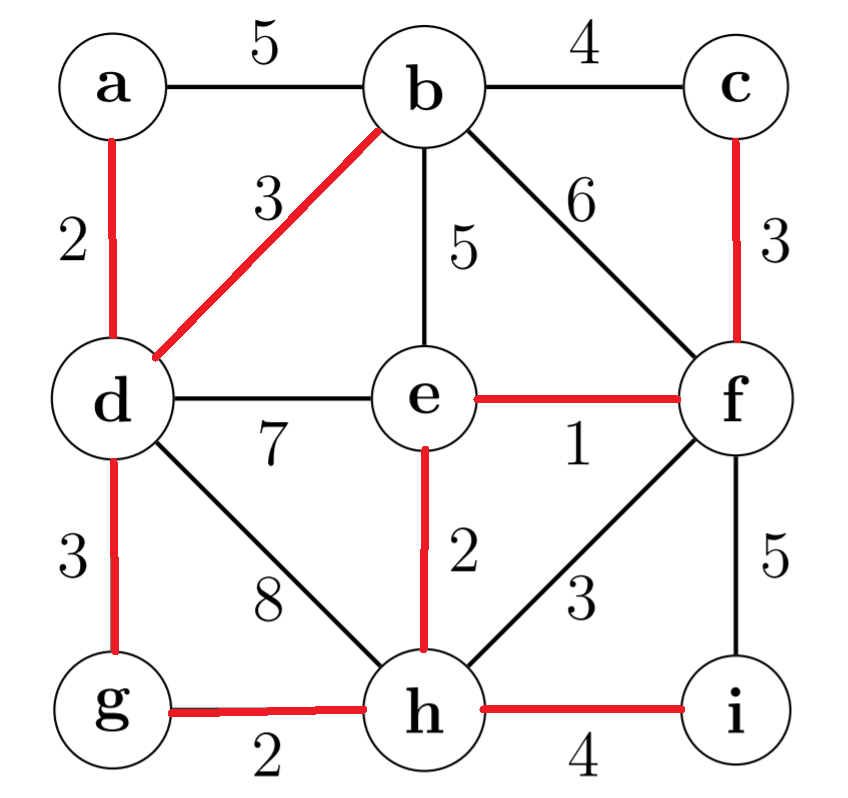
\includegraphics[scale=0.35]{annenspanningtree.png}\\
\end{center}
c) For graph G, there is a unique minimum spanning tree. Even if we change the order we chose the the least edge, we end up in the same spanning tree. However, in general this is not the case. There may be more than one spanning trees whenever there are more than one equivalent edges to select among. Different choices may yield different spanning trees.\\
d) Let the graph G have a unique minimum-weight edge e, which connects vertices a and b. Assume that there is a spanning tree T, that does not include edge e. If we add e to T, then we will obtain a graph with exactly one simple circuit, which contains e. Then we can delete some other edge in this circuit resulting in a spanning tree with weight strictly less than T since all the weights are greater than edge e's weight. This contradicts with the assumption at the beginning, T is the minimum-spanning tree. Since we reached a contradiction we can conclude that our assumption is false. In other words, if the minimum-weight edge of a graph is unique, then this edge is included in any minimum spanning tree for that graph.\\
\section*{Answer 2}
There is at least one mapping from graph G to graph H: (a, b, c, d, e, f) $\rightarrow$ (n, q, o, r, m, p). Since there exists a mapping from G to H, G and H are isomorphic.

\section*{Answer 3}
a) The number of vertices: 7\\
The number of edges: 6\\
Height: 3\\\\
b) Postorder traversal: q, s, u, v, t, r, p\\
Inorder traversal: q, p, s, r, u, t, v\\
Preorder traversal: p, q, r, s, t, u, v\\\\
c) T is a full binary tree because all of its nodes have either zero or two children.\\\\
d) T is not a complete binary tree because before the level 2 was filled, level 3 was started to be filled.\\\\
e) T is not a balanced tree because the difference between the depth of left subtree and the right subtree of node p is 2 (which is greater than 1).\\\\
f) In a binary search tree, by convention, the node values in the rightern subtree of a node are greater that the node's, and the node values in the leftern subtree of a node are smaller than the node's. Since in tree T, value of node u (23), is smaller than that of node r (24), tree T cannot be a binary search tree.\\\\
g) Let U be a full binary tree with height n. Since every node will have either two or zero children; for it to have minimum number of nodes, it should have 2 nodes at every level; except for the level 0, which has only one node. Since there are height+1 levels, the general formula for the minimum number of nodes is:\\ minimum number of nodes = 2*n + 1\\
If n = 5, minimum number of nodes is 2*5 + 1 = 11.\\


\end{document}